Up to this chapter, our focus has been on the fullfillment of a constraint given in terms of production rate and production time. In this part of the course, we will change our main objective by adding a constraint on the number of items to be produced. Still we will have a minimum rate to be performed, stil we will have a production time limit not to be crossed, but the objective now becomes to produce exactely $N$ final products and to plan the production accordingly. 

\section{Given that $b_i = b_fn_{if}$}

We know, from the previous chapters, that the production time can be computed as \[ T_{prod}(b_f) = \max_{\mathcal P_k}\left( \sum_{i\in\mathcal P_k}(T_{si} + b_fT_{oi}n_{if}) \right) \] but it is worthy to notice that the time to seperately produce two batches of size $b_f$ does not equal the double time we would need to produce one batch of size $b_f$. More formally, we are saying that $T_{prod}(2.b_f)|_{b_f}\ne 2T_{prod}(b_f)$ in the sense that figure (\ref{produced_i:2bf}) represents. In fact, we do not need for a whole "production cycle" to be finished to begin with another one. Indeed, we can begin a new cycle as soon as the "longest" machine has done its work (i.e. the bottleneck machine). The following formula holds instead : \[ \left. T_{prod}(2.b_f) \right|_{b_f} = T_{prod}(b_f) + T_b(b_f) \] where $\left. T_{prod}(2.b_f) \right|_{b_f}$ represents the time needed to produce $2.b_f$ items knowing that the batch size is $b_f$ and where $T_b(b_f)$ is the time which is needed, by the bottleneck machine (hence $T_b$ for bottleneck) to produce a bacth of size $b_f$. This formula can, for sure, be generalized as \begin{equation} \left. T_{prod}(K.b_f) \right|_{b_f} = T_{prod}(b_f) + (K-1)T_b(b_f) \label{produced_i:tprod} \end{equation}

\begin{figure}[h!]
    \centering
    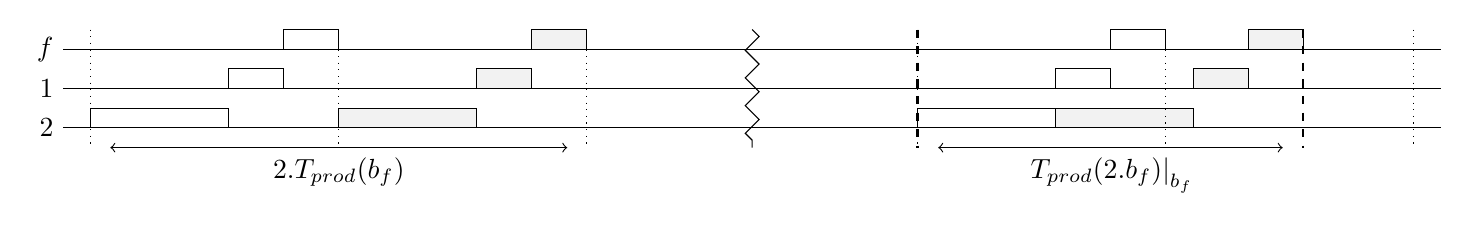
\begin{tikzpicture}[xscale=.7, yscale=.5]
        \draw (0,0) node[left] {$f$} -- (25, 0);
        \draw (0,-1) node[left] {$1$} -- (25, -1);
        \draw (0,-2) node[left] {$2$} -- (25, -2);
        \draw[decorate, decoration=zigzag] (12.5, .5) -- (12.5, -2.5);

        % left
        \draw (.5, -2) rectangle (3, -1.5);
        \draw (3, -1) rectangle (4, -.5);
        \draw (4, 0) rectangle (5, .5);

        \draw[fill=gray!10] (5, -2) rectangle (7.5, -1.5);
        \draw[fill=gray!10] (7.5, -1) rectangle (8.5, -.5);
        \draw[fill=gray!10] (8.5, 0) rectangle (9.5, .5);

        \draw[dotted] (.5, .5) -- (.5, -2.5) node[right] (l1) {};
        \draw[dotted] (5, .5) -- (5, -2.5);
        \draw[dotted] (9.5, .5) -- (9.5, -2.5) node[left] (l2) {};

        \draw[<->] (l1) -- node[below] {$2.T_{prod}(b_f)$} (l2);

        % right
        \draw (15.5, -2) rectangle (18, -1.5);
        \draw (18, -1) rectangle (19, -.5);
        \draw (19, 0) rectangle (20, .5);

        \draw[fill=gray!10] (18, -2) rectangle (20.5, -1.5);
        \draw[fill=gray!10] (20.5, -1) rectangle (21.5, -.5);
        \draw[fill=gray!10] (21.5, 0) rectangle (22.5, .5);

        \draw[dotted] (15.5, .5) -- (15.5, -2.5);
        \draw[dashed, thick] (15.5, .5) -- (15.5, -2.5) node[right] (r1) {};
        \draw[dashed, thick] (22.5, .5) -- (22.5, -2.5) node[left] (r2) {} ;
        \draw[dotted] (20, .5) -- (20, -2.5);
        \draw[dotted] (24.5, .5) -- (24.5, -2.5);

        \draw[<->] (r1) -- node[below] {$\left. T_{prod}(2.b_f)\right|_{b_f}$} (r2);

    \end{tikzpicture}
    \caption{\label{produced_i:2bf}}
\end{figure}

\subsection{A first example}

However, the above formula holds for a given bottleneck machine. But we do know that the bottleneck machine depends on the batch size which has been chosen \textit{a priori} : given a batch size $b_f$, we can comptue the production time $T_{prod}(K.b_f)|_{b_f}$. But how can we choose $b_f$ with constraints on the production rate, on the overall production time, and, as well, on the number of items to be produced ? This is not an easy question actually, so let's take an example in order to better understand where the difficulty lies. 

\begin{wrapfigure}[12]{r}{5cm}
    \centering
    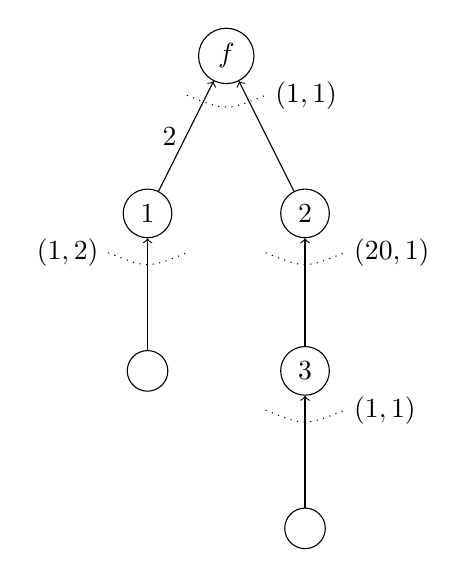
\begin{tikzpicture}
        \draw (0,0) node[draw, circle] (f) {$f$};
        \draw (-1, -2) node[draw, circle] (1) {$1$};
        \draw (-1, -4) node[draw, circle] (RM1) {$\vphantom{1}$};

        \draw (1, -2) node[draw, circle] (2) {$2$};
        \draw (1, -4) node[draw, circle] (3) {$3$};
        \draw (1, -6) node[draw, circle] (RM2) {$\vphantom{1}$};

        \draw[->] (RM1) -- (1);
        \draw[->] (1) -- node[left] {$2$} (f);

        \draw[->] (RM2) -- (3);
        \draw[->] (3) -- (2);
        \draw[->] (2) -- (f);

        \draw[dotted] (-.5, -.5) .. controls (0, -.7) .. (.5, -.5) node[right] {$(1, 1)$};
        \draw[dotted] (-1.5, -2.5) node[left] {$(1, 2)$} .. controls (-1, -2.7) .. (-.5, -2.5);
        
        \draw[dotted] (.5, -2.5) .. controls (1, -2.7) .. (1.5, -2.5) node[right] {$(20, 1)$};
        \draw[dotted] (.5, -4.5) .. controls (1, -4.7) .. (1.5, -4.5) node[right] {$(1, 1)$};
    \end{tikzpicture}
    \caption{\label{produced_i:example1}Example BoM}
\end{wrapfigure}

Let's consider the Bill of Material depicted in figure (\ref{produced_i:example1}) with the following constraints : \begin{enumerate}
    \item Minimum production rate of $X_f^* = \frac{1}{5}$
    \item Maximum production time for a batch $\bar T = 80$
    \item Number of items to be produced $N = 200$
\end{enumerate} We are very used to the first two constraints. The first one gives us a lower bound for the batch size in order for the production rate to be feasible. The second one gives us an upper bound so that the production time of a batch is not greater than the time limit. Computing these bounds is rather easy and we will not discuss them : 
\[
    \begin{split}
        b_f^* &= \max_i\left( \frac{X_f^*T_{si}}{1-X_f^*T_{oi}n_{if}} \right)\\
              &= \max\left(
                    \frac{ \frac{1}{5} . 1 }{1 - \frac{1}{5} . 1 } ;
                    \frac{ \frac{1}{5} . 1 }{1 - \frac{1}{5} . 2 . 2 } ;
                    \frac{ \frac{1}{5} . 20 }{1 - \frac{1}{5} . 1 . 1 } ;
                    \frac{ \frac{1}{5} . 1 }{1 - \frac{1}{5} . 1 . 1 }
                  \right)\\
              &= 5\\
        \bar b_f &= \min_{\mathcal P_k}\left( \frac{\bar T - \sum_{i\in\mathcal P_k}T_{si}}{\sum_{i\in\mathcal P_k}T_{oi}n_{if}}\right)\\
                 &= \min\left(
                        \frac{80 - ( 1 + 1 )}{ 2.2 + 1.1 } ;
                        \frac{80 - ( 1 + 20 + 1 )}{ 1.1 + 1.1 + 1.1 } ;
                    \right)\\
                 &= 15.6
    \end{split}
\]

Which tells us that we need to choose our batch size so that $b_f\in [ 5, 15 ]$. Since we want to produce $N=200$ items, we should repeat a certain number of times the production of such bacthes untill we reach $200$ items. On possible way would be to produce $40$ times a batch of $5$ items (since $40\times 5 = 200$), or produce $25$ times batches of $8$ (since again $25\times 8=200$). In fact, the only multiples of $200$ witin the interval $[5, 15]$ are $\{ 5, 8, 10 \}$. Let's study each one of these cases !

For each cases, we can write the equation (\ref{produced_i:tprod}) as \[
    \begin{split}
        T_{prod}(200)|_{bf=5} &= T_{prod}(5) + 39.T_b(5)\\
        T_{prod}(200)|_{bf=8} &= T_{prod}(8) + 39.T_b(10)\\
        T_{prod}(200)|_{bf=10} &= T_{prod}(8) + 39.T_b(10)\\
    \end{split}
\] where $T_{prod}(b_f)$ can be computed as \[
    T_{prod}(b_f) = \max_{\mathcal P_k}\left( \sum_{i\in\mathcal P_k} ( T_{si} + T_{oi}n_{if} ) \right) = \max ( 2 + 5.b_f ; 22 + 3.b_f )
\] and \[ T_b(b_f) = \max( 1 + 1.b_f ; 1 + 2.2.b_f ; 20 + 1.b_f ; 1 + 1.b_f ) = \max( 1 + 4b_f ; 20 + b_f ) \]

Using these formulas, we easily get the following results : \begin{center}
    \begin{tabular}{|c|c|c|c|}
        \hline
        $b_f$ & $T_{prod}(b_f)$ & $T_b(b_f)$ & $T_{prod}(200)|_{b_f}$\\\hline
        $5$ & $37$ & $25$ & $1012$ \\\hline
        $8$ & $46$ & $33$ & $838$ \\\hline
        $10$ & $52$ & $41$ & $831$ \\\hline
    \end{tabular}
\end{center} Which means that, for this way of producing $200$ items, using a batch size of $10$ items is the quicker (it turns out to be the biggest batch size but this is just a particular case). However, there are other ways of getting to $200$ ! For example, we may want to produce $13$ batches of $15$ and a batch of $5$, since $200 = 13\times 15 + 5$. Looking at figure (\ref{produced_i:gant}), we realise that we can compute the time needed to produce $200$ items in that way by first computing the time to produce $13$ bacthes of $15$ and then add the difference between the needed time to produce a batch of $5$ and the time at which the bottleneck machine can start.

We get that : \[
    \begin{split}
        T_{prod}(15) &= 77\\
        T_b(15) &= 61\\
        T_{prod}(195)|_{bf=15} &= 77 + 12.61 = 809\\
        T_{prod}(5) &= 37\\
        T_b(5) &= 25
    \end{split}
\] And, it holds that the delay represented by the red arrow in figure (\ref{produced_i:gant}) can be computed as the production time of the bottleneck machine $T_b(5)$ minus the production time of machine $f$, which yields $25 - 16 = 9$. We can now compute the final, overall, production time which is : $809 + 9 + 6 = 824$ ! Which is less than what we had previously found. 

\begin{figure}[h!]
    \centering
    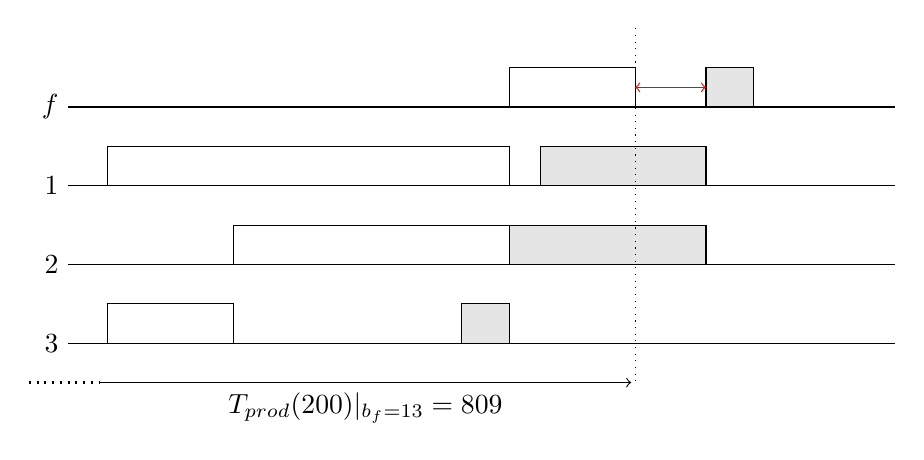
\begin{tikzpicture}[xscale=.1]
        \foreach \y/\m in {0/$f$, -1/$1$, -2/$2$, -3/$3$} \draw (-5,\y) node[left] {\m} -- (100, \y);

        \draw (0,-3) rectangle (16, -2.5);
        \draw (16,-2) rectangle (16 + 35, -1.5);
        \draw (0,-1) rectangle (51, -.5);
        \draw (51, 0) rectangle (51 + 16, .5);

        \draw[fill=gray!20] (51, -2) rectangle (51 + 25, -1.5);
        \draw[fill=gray!20] (51 + 25 - 21, -1) rectangle (51 + 25, -.5);
        \draw[fill=gray!20] (51 - 6, -3) rectangle (51, -2.5);
        \draw[fill=gray!20] (51 + 25, 0) rectangle (51 + 25 + 6, .5);

        \draw[dotted] (67, 1) -- (67, -3.5);

        \draw[->] (-1, -3.5) -- node[below] {$T_{prod}(200)|_{b_f = 13} = 809$} (66.5, -3.5);
        \draw[dotted, thick] (-10, -3.5) -- (-1, -3.5);
        
        \draw[<->, red] (67, .25) -- (67 + 9, .25);
    \end{tikzpicture}
    \caption{\label{produced_i:gant}GANT diagram corresponding to the production of $200 = 13\times 15 + 5$ items}
\end{figure}

Finding the optimal batch size is not easy to be done by hand and we usually use approximation techniques to find a solution. 

\subsection{Approximate solution}

Let us define our coefficient $K$ as $\frac{N}{b_f}$ and let's assume that this number is an integer number. Then, assuming that we know \textit{a priori} the bottleneck machine $b$, it holds that \[ \begin{split}
    T_{prod}(N)|_{b_f} &= \sum_{i\in\mathcal P_k} ( T_{si} + T_{oi}n_{if}b_f ) + \left( \frac{N}{b_f} - 1 \right)(T_{sb} + b_fT_{ob}n_{bf})\\
    &= \sum_{i\in\mathcal P_k} T_{si} + b_f\left( \sum_{i\in\mathcal P_k} T_{oi}n_{if} - T_{ob}n_{bf} \right) + NT_{ob}n_{bf} + \frac{N}{b_f}T_{sb}
    \end{split}
\] which is just a re-writing of the previously introduced equations. This function of $b_f$ is convex, we can find its global minimum by first relaxing the "integer" constraint and derivating this function and solving $\nabla . = 0$. We get
\[
    \frac{\partial .}{\partial b_f} = \sum_{i\in\mathcal P_k} T_{oi}n_{if} - T_{ob}n_{bf} - \frac{N}{b_f^2}T_{sb}
\] and \[
    \nabla . = 0 \Leftrightarrow b_f^\circ = \sqrt{ \frac{T_{sb}}{\sum_{i\in\mathcal P_k} T_{oi}n_{if} - T_{ob}n_{bf} } }
\]
This results gives us the optimal batch size we should use \textbf{given the bottleneck machine considered}. However, we know that the bottleneck changes with the batch size. In fact, imagine a situation in which the bottleneck machine changes for a given batch size, say $\tilde b_f$. And imagine a situation in which, for $b_f > \tilde b_f$, we have a convex function like the red one in figure (\ref{produced_i:convex}), and that, on the other hand, for $b_f < \tilde b_f$, we have a convex function like the black one in the same figure. Using that formula will yield one of the two extremum depending on which machine we assume to be the bottleneck machine...

\begin{figure}[h!]
    \centering
    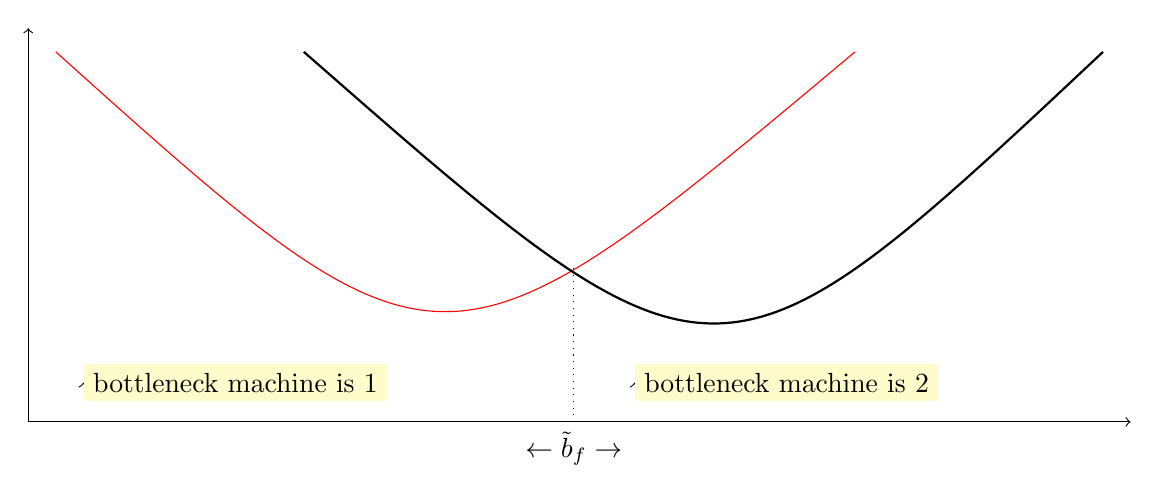
\begin{tikzpicture}[xscale=.7]
        \draw[<->] (0, 5) |- (20, 0);

        \draw[->] (1, .5) node[fill=yellow!20, right] {bottleneck machine is $1$};
        \draw[->] (11, .5) node[fill=yellow!20, right] {bottleneck machine is $2$};

        \draw[red] (0.5, 4.7) .. controls (7.5, .3) .. (15, 4.7);
        \draw[thick] (5, 4.7) .. controls (12.5, .1) .. (19.5, 4.7);
        \draw[dotted] (9.9, 0) node[below] {$\leftarrow\tilde b_f\rightarrow$} -- ++(0, 1.95);
    \end{tikzpicture}
    \caption{\label{produced_i:convex}Two different convex functions for finding "optimal" batch size}
\end{figure}

\section{Arbitrary batch sizing}
